\subsubsection{Overview / description/parameters}
%Describe concept of accumulator pack, provide table with main parameters like number of cells, cell stacks separated by maintenance plugs, cell configuration, resulting voltages->minimum, maximum, nominal, currents, capacity etc.
Our accumulator pack is designed using 18650 Li-ion cells in 6 stacks configuration, active cooled by air. The accumulator pack contains cells, \gls{ams} modules (slaves), \gls{acp} main control unit (\gls{ams} master) with DC/DC converter, \gls{imd} unit, cooling fans and current sensor. There is smaller insulated box inside the accumulator pack, that accomodates \glspl{air} and main fuse.
Details are filled in following table:

\begin{table}[H]
	\centering
	\caption{Main accumulator parameters}
	\begin{tabu}{|X|X|}
		\hline
		Maximum Voltage: & 400 $V_{DC}$ \\
		\hline
		Nominal Voltage: & 345.6 $V_{DC}$ \\
		\hline
		Minimum Voltage: & 182 $V_{DC}$ \\
		\hline
		Maximum output current: & 315 A (until any cell reaches 80 $^\circ$C) \\
		\hline
		Maximum nominal current: & 270 A \\
		\hline
		Maximum charging current: & 54 A \\
		\hline
		Total numbers of cells: & 864 \\
		\hline
		Cell configuration: & 96s9p \\
		\hline
		Total Capacity: & 27.99 MJ \\
		\hline
		Number of cell stacks < 120 $V_{DC}$ & 6 \\
		\hline
	\end{tabu}%
	\label{tab:acc-main}%
\end{table}%

\subsubsection{Cell description}
%Describe the cell type used and the chemistry, provide table with main parameters.

The used cell is the 18650 type cylindrical Li-ion cell. Detailed specification is shown in table below. Each cell has a \gls{cid} which disconnect the cell from others in parallel in case of cell failure (such an internal short circuit or over pressure) or in case of excessive discharge current. 

\begin{table}[H]
	\centering
	\caption{Main cell specification}
	\begin{tabu}{|X|X|}
		\hline
		Cell Manufacturer and Type & SONY VTC5A \\
		\hline
		Cell nominal capacity: & 2.5 Ah \\
		\hline
		Maximum Voltage: & 4.25 V \\
		\hline
		Nominal Voltage: & 3.6 V \\
		\hline
		Minimum Voltage:  & 2 V \\
		\hline
		Maximum output current: & 35 A (until cell reaches 80 $^\circ$C) (14C)\\
		\hline
		Maximum nominal output current: & 30 A(12C) \\
		\hline
		Maximum charging current: & 6 A(2.4C) \\
		\hline
		Maximum Cell Temperature (discharging) & 80 $^\circ$C \\
		\hline
		Maximum Cell Temperature (charging) & 60 $^\circ$C \\
		\hline
		Cell chemistry: & Lithium-Ion \\
		\hline
	\end{tabu}%
	\label{tab:acc-cell}%
\end{table}%

\subsubsection{Cell configuration}
%Describe cell configuration, cell interconnect, show schematics of electrical configuration and CAD of connection techniques, cover additional parts like internal cell fuses etc.

Cell configuration is 96s9p. Cells are divided into 6 stacks, configuration of each stack is 16s9p. Cells are connected by welding. Main cells interconnection is done by nickel sheet. This sheet is welded to each cell. There is additional copper sheet welded over the nickel sheet (for lowering resistance of the main current path).

 
\subsubsection{Cell temperature monitoring}
%Describe how the temperature of the cells is monitored, where the temperature sensors are placed, how many cells are monitored, etc. Show schematics, cover additional parts, etc.

	The cells’ temperature is monitored by \gls{ntc} temperature sensors. The manufacturer is TDK, type is: B57330V2103F260. Insulation of the sensors is done by 3M\textsuperscript{TM} PTFE Film Electrical Tape. Breakdown voltage of this tape 9.5 kV, operating temperature is 180 $^\circ$C. Thickness of this tape is 0.1 mm. Sensors are soldered in \glspl{pcb} that are covered with insulating tape and then mounted to each stack. 

\begin{figure}[H]
	\centering
	\includegraphics[width=\textwidth]{./img/ACP-stack.png}
	\caption{Stack configuration.}
	\label{fig:acp-stack}
\end{figure}

Position of temperature sensors on the top of each stack (highlighted objects)
\begin{figure}[H]
	\centering
	\includegraphics[width=\textwidth,trim={0cm 16cm 0cm 0cm}, clip]{./img/BMS-top-sensors.pdf}
	\caption{Top position of sensors.}
	\label{fig:bms-top}
\end{figure}
Position of temperature sensors on the bottom of each stack (highlighted objects)
\begin{figure}[H]
	\centering
	\includegraphics[width=\textwidth,trim={0cm 16cm 0cm 0cm}, clip]{./img/BMS-bottom-sensors.pdf}
	\caption{Bottom position of sensors.}
	\label{fig:bms-bottom}
\end{figure}
Top and bottom view of one stack 
\begin{figure}[H]
	\centering
	\includegraphics[width=\textwidth]{./img/BMS-top-andbottom.pdf}
	\caption{Rear and bottom view.}
	\label{fig:bms-top-and-bottom}
\end{figure}

\begin{table}[H]
	\centering
	\caption{General cell temperature parameters.}
	\begin{tabu}{|X|X|}
		\hline
		Temperature sensor accuracy: & 1\% \\
		\hline
		Total number of cells: & 864 \\
		\hline
		Total number of sensors: &  384 \\
		\hline
		Max. distance from monitored negative cell terminal: & 2 mm \\
		\hline
		\gls{ams} opens \glspl{air} during dis-charging if cell temperature is above: & 60 $^\circ$C \\
		\hline
		\gls{ams} opens \glspl{air} during charging if cell temperature is above: & 60 $^\circ$C \\
		\hline
	\end{tabu}%
	\label{tab:acc-temp}%
\end{table}%

\subsubsection{Accumulator Management System}\label{subsec:ams}
%Describe the \gls{ams} used including at least the following:

In our \gls{ams} system, we use the bq76PL455A-Q1 device that is an integrated 16-cell battery monitoring and protection device, designed for high-reliability automotive applications. The communication is high-speed, differential, capacitor-isolated and allows to communicate with a host via a single high-speed Universal Asynchronous Receiver/Transmitter (UART) interface.
The bq76PL455A-Q1 monitors and detects several different fault conditions, including: overvoltage, undervoltage, overtemperature, and communication faults. Six GPIO ports as well as eight analog AUX \gls{adc} inputs (that are externally multiplexed to measure temperature of almost half of the cells) are included for additional monitoring. A secondary thermal shutdown is included for further protection. \ref{app:bms_datasheet}

\begin{table}[H]
	\centering
	\caption{Cell voltage limits.}
	\begin{tabu}{|X|X|}
		\hline
		Minimum cell voltage (shutdown limit): & 2.2 V \\
		\hline
		Maximum cell voltage (shutdown limit): & 4.2 V \\
		\hline
		Measurement precision (mV): & $\pm$ 0.75 \\
		\hline
	\end{tabu}%
	\label{tab:acc-limits}%
\end{table}%

%\item Sense wiring protection (fusing / fusible link wire used)
%\item What upper and lower voltage does the AMS react at and how does it react?
%\item What cell temperature does the AMS react at and how does it react?
%\item Show tables of operation parameters
%\item Describe how many cells are sensed by each AMS board, the configuration of the cells, the configuration of the boards and how any communications wiring between boards is protected 
%\item Describe how the AMS is able to open the AIRs if any error is detected
%\item Describe where galvanic isolation occurs between TS and GLV system connections.

Each sense connection is protected with fuse. There are two types of fuses used: 

\noindent Littelfuse 0251001.MXL (Those are used, where the cells are contacted via \gls{pcb})

\noindent Eaton TR/3216LV1-R (Those are used, where measure wires are connected directly to cells)

Cell highest allowed voltage is 4.25 V so \gls{ams} reacts when the voltage is above 4.2 V. Cell lowest allowed voltage is 2 V so \gls{ams} reacts when the voltage is below 2.2 V. Reaching any of limits causes \glspl{air} disconnection.

Highest allowed temperature (by datasheet) for discharging is 80 $^\circ$C and for charging 60 $^\circ$C. Due to FSE rules our battery pack is limited to 60 $^\circ$C. \gls{ams} reacts when the temperature is higher than 60 $^\circ$C and causes \glspl{air} disconnection.

\paragraph{Recommended Operating Conditions}
TA = 25 $^\circ$C and TOP = 57.6 V; Min/Max values stated where TA = -40 $^\circ$C to 105 $^\circ$C and TOP = 12 V to 79.2 V (unless otherwise noted)
\begin{figure}[H]
	\centering
	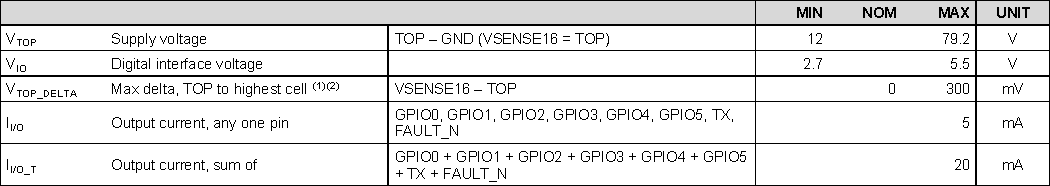
\includegraphics[width=\textwidth]{./img/BMS-operatingparms.pdf}
	\caption{Recommended operating parameters.}
	\label{fig:BMS-op-params}
\end{figure}


Each \gls{ams} board senses whole stack, that means it senses 144 cells, connected in 16s9p configuration. Communications wirings are protected by two 1kV 1nF capacitors CC1206KKX7RCBB102 by Yageo. There is placed one on each side (there is one on every \gls{ams}). The \gls{ams} is connected to Accumulator \gls{ecu} that has capability of direct \glspl{air} shutdown. The galvanic isolation between \gls{ts} and \gls{glvs} is done by two 1kV 1nF capacitors CC1206KKX7RCBB102 by Yageo. It is located on separated board connected between first \gls{ams} and Accumulator \gls{ecu}.




\subsubsection{Accumulator indicator}
%Describe the indicator, show wiring, provide tables with operation, PCB design, etc

We use LED indicator placed on Accumulator pack chassis. The LED is powered by a separate circuit which is also used to power the \gls{tsal}. The circuit function explanation is shared with \gls{tsal} HV part. 

\subsubsection{Wiring, cables, current calculations, connectors}\label{subsec:acp_wiring}
%Describe the internal wiring, show schematics, provide calculations for currents and voltages and show data regarding the cables and connectors used.
%	\item 	Discuss maximum expected current, DC and AC how long will this be provided?
%	\item Compare the maximum values to nominal currents
%	\item Give a table for each kind of wire in your tractive-system:
%	\item Describe your maintenance plugs, provide pictures
%	\item Use tables like the one shown below:


We use OLFLEX HEAT 180 SiF (see. \ref{app:PowerConductor})as Tractive System wires. Total gauge is 16mm2. Total ampacity is 165 A for main DC power buses. All other LV wiring in Accumulator is also done using OLFLEX HEAT 180 SiF wires with gauges ranging from 0,25 mm$^2$ to 1 mm$^2$. Basic data are given in tables below. We use 2 pin Deutsch ASHD connectors as \gls{ts} connectors as the Accumulator Pack outlet, Service box inlet and Motor controllers inlet. For Motor controllers outlets to motors we use 4 pin Deutsch ASHD connectors. Pins are rated each to 200 A of continuous current. According to our data from last season, average continuous DC current is expected to be around 80 A. The maximum DC current should be 250 A for 5 seconds at maximum.

To ensure that connectors will withstand in-rush currents, we did following calculation. The most stressed connector is Accumulator pack outlet. The maximum power, Motor Controllers will take, is 80kW, which is 250A in maximum (depends on state of charge of accumulators). Based on heating, thermal capacity of mass of pins and nearest wiring, by power losses on contact resistance and temperature difference 50 $^\circ$C, these connectors will definitely withstand this current for more than 10 seconds, which is far ahead of motors overload capacity (cca. 4-5 seconds). Therefore, these connectors will never reach critical overload condition.


% Table generated by Excel2LaTeX from sheet 'List1'
\begin{table}[htbp]
	\centering
	\caption{Wire data of company A, 0.205 mm$^2$.}
	\begin{tabu}{|X|X|}\hline
		Wire type & OLFLEX HEAT 180 SiF \\\hline
		Continuous current rating: & 165 A \\\hline
		Cross-sectional area & $16mm^2$ \\\hline
		Maximum operating voltage: &  500 V$_{DC}$\\\hline
		Temperature rating: &  125 $^\circ$C\\\hline
		Wire connects the following components: & Stacks $\,\to\,$ \glspl{air}, fuse $\,\to\,$ \gls{hv} Connector \\\hline
	\end{tabu}%
	\label{tab:acc-wire}%
\end{table}%

\begin{figure}[H]
	\centering
	\includegraphics[width=\textwidth]{./img/ACP-nut.png}
	\caption{Maintenance plugs I.}
	\label{fig:acp-maintance-plug}
\end{figure}

\begin{figure}[H]
	\centering
	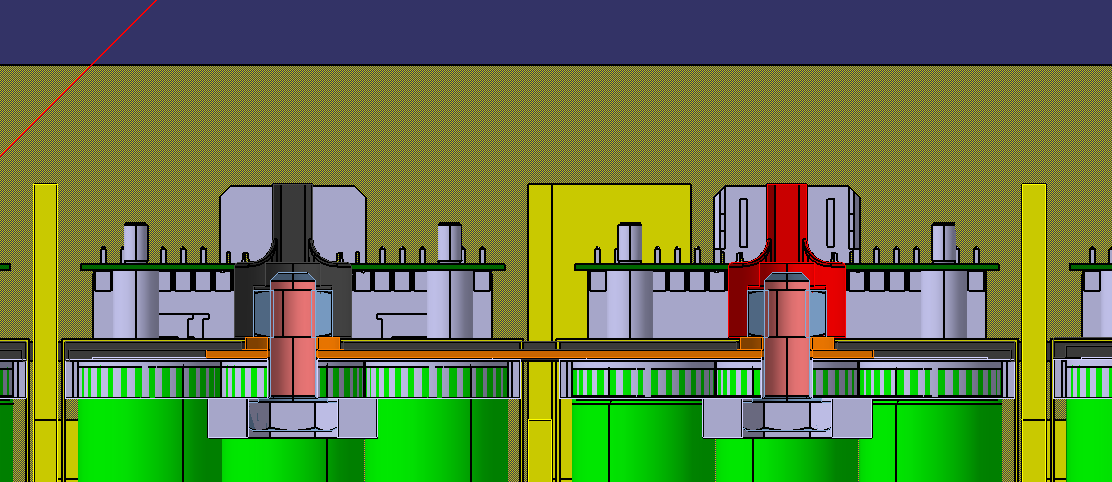
\includegraphics[width=\textwidth]{./img/ACP-nut2.png}
	\caption{Maintenance plugs II.}
	\label{fig:acp-maintance-plug2}
\end{figure}

\begin{figure}[H]
	\centering
	\includegraphics[width=\textwidth]{./img/ACP-view.png}
	\caption{Accumulator pack \gls{hv} wiring I.}
	\label{fig:acp-hv-wiring}
\end{figure}

\begin{figure}[H]
	\centering
	\includegraphics[width=\textwidth]{./img/ACP-fuse.png}
	\caption{Accumulator pack \gls{hv} wiring II.}
	\label{fig:acp-hv-wiring2}
\end{figure}

\subsubsection{Accumulator insulation relays}\label{subsec:airs}
%Describe the AIRs used and their main operation parameters, use tables, etc.

We use Kilovac EV200 as \glspl{air}, it is widely used standard contactor designed for EVs, working with inert gas atmosphere. Detailed specification is given in the following table:

% Table generated by Excel2LaTeX from sheet 'List1'
\begin{table}[H]
	\centering
	\caption{Basic AIR data.}
	\begin{tabu}{|X|X|}
		\hline
		Relay Type: & Kilovac EV200 \\
		\hline
		Contact arrangement: & SPST \\
		\hline
		Continuous DC current rating: & 500 A \\
		\hline
		Overload DC current rating:  & 2000 A for 1 second \\
		\hline
		Maximum operation voltage: & 900 V$_{DC}$ \\
		\hline
		Nominal coil voltage: & 24 V$_{DC}$ \\
		\hline
		Normal Load switching: & Make and break up to 650 A \\
		\hline
		Maximum Load switching & 3 times at 2000 A \\
		\hline
	\end{tabu}%
	\label{tab:acc-air}%
\end{table}%

\subsubsection{Fusing}
%Describe the fuses used and their main operation parameters, use tables, etc.
%Additionally, fill out the following table for each fuse type used:

We use OEZ Varius P51T06 as the main fuse. It is intended to protect semiconductors. Both contactors and main fuse are enclosed in separate enclosure as it can be seen in the pictures above. Detailed specification is given in the following table:

\begin{table}[H]
	\centering
	\caption{Basic fuse data}
	\begin{tabu}{|X|X|}
		\hline
		Fuse manufacturer and type: & OEZ Varius P51T06 160A aR \\
		\hline
		Continuous current rating:  & 160 A \\
		\hline
		Maximum operating voltage  & 440 V$_{DC}$ \\
		\hline
		Type of fuse: & High speed for semiconductors \\
		\hline
		I2t rating: & 3300 A$^{2}$s \\
		\hline
		Interrupt Current (maximum current at which the fuse can interrupt the current) & 50 kA \\
		\hline
	\end{tabu}%
	\label{tab:acc-fuse}%
\end{table}%

%Create a table with components and wires protected by the fuse(s) and the according continuous current rating, below is an example table with some potential entries.  Complete this table with information for your design and add/remove additional locations as applicable.  Ensure that the rating of all the components is greater than the rating of the fuse such that none of the other components become the fuse.

%\todo[inline]{Tohle je ještě potřeba vyplnit!}

% Table generated by Excel2LaTeX from sheet 'List1'
\begin{table}[H]
	\centering
	\caption{Fuse Protection Table}
	\begin{tabu}{|X|X|X|X|X|}
		\hline
		Location & Wire Size & Wire Ampacity & Fuse type & Fuse rating\\
		\hline
		Cells to AIRs & 6 AWG & 165 A & High-speed & 160 A \\
		\hline
		AIR to Motor controller & 6 AWG & 165 A & High-speed & 160 A \\
		\hline
		AIR to TSAL & 22 AWG & 5 A & High-speed & 3 A \\
		\hline
		Accumulator output connector & 6 AWG & 165 A & High-speed  & 160 A \\
		\hline
		Cells to AMS & N/A (PCB trace) & 5 A    & SMD    & 2 A \\
		\hline
	\end{tabu}%
	\label{tab:acc-fuse-protection}%
\end{table}%

\subsubsection{Charging}
We use self developed charger to charge our accumulator pack. Figure \ref{fig:charger_topology} shows the charger concept. It is comprised of galvanically isolated step-up transformer, followed by step-down converter. Charger is connected to the accumulator pack by a separate low voltage and high voltage connectors. CAN bus is used for data communication, which goes through the low voltage cord. 

Charger is equipped with properly designed Shutdown Circuit, and several safety features. The overall shutdown circuit through the charger is in \ref{fig:charger_sdc_scheme}. The \gls{sdc} begins in the charger and goes through the charger's shutdown button SB1. Kd is a door switch of the electrical panel, S$_1$ is a software controlled relay that needs to be closed first in order to start the charging process. S$_1$ is closed after the charger goes through a self-test. Charging is started by pressing SB$_2$, which is the charging start button. If the \gls{sdc} is completed through all safety checks (including connector interlocks on the charger and \gls{acp}, also \gls{imd} and \gls{ams}, the charging process is started. The charging process is fully automatic. Voltage and current is dictated by the \gls{acp} \gls{ams} system (\gls{ecua}) and negotiated through the CAN bus.

Charger HV output is fused in both poles, using a 32 A fuse. (\ref{app:charger_fuse_datasheet}) For additional safety, charger \gls{hv} output terminals are switched using two contactors, same type as the \gls{acp} \glspl{air} (\ref{app:air_datasheet}). Charger output terminals are isolated by the charger isolation relays whenever the \gls{sdc} is interrupted. The step-down converter in the charger contains significant dc-link capacitance, that is always discharged using the KM$_4$ contactor. The KM$_4$ contactor is a normally closed type and controlled by a hardwired contact logic.

Note: The Ix denoted points in the \ref{fig:charger_sdc_scheme} are signals for the charger control unit, to sense the state of the \gls{sdc}. The Sx denoted contacts are software controlled relays from the charger control unit.

\ref{fig:charger_layout} shows proper isolation gaps are always maintained on the \gls{hv} circuitry.


\begin{figure}[H]
	\centering
	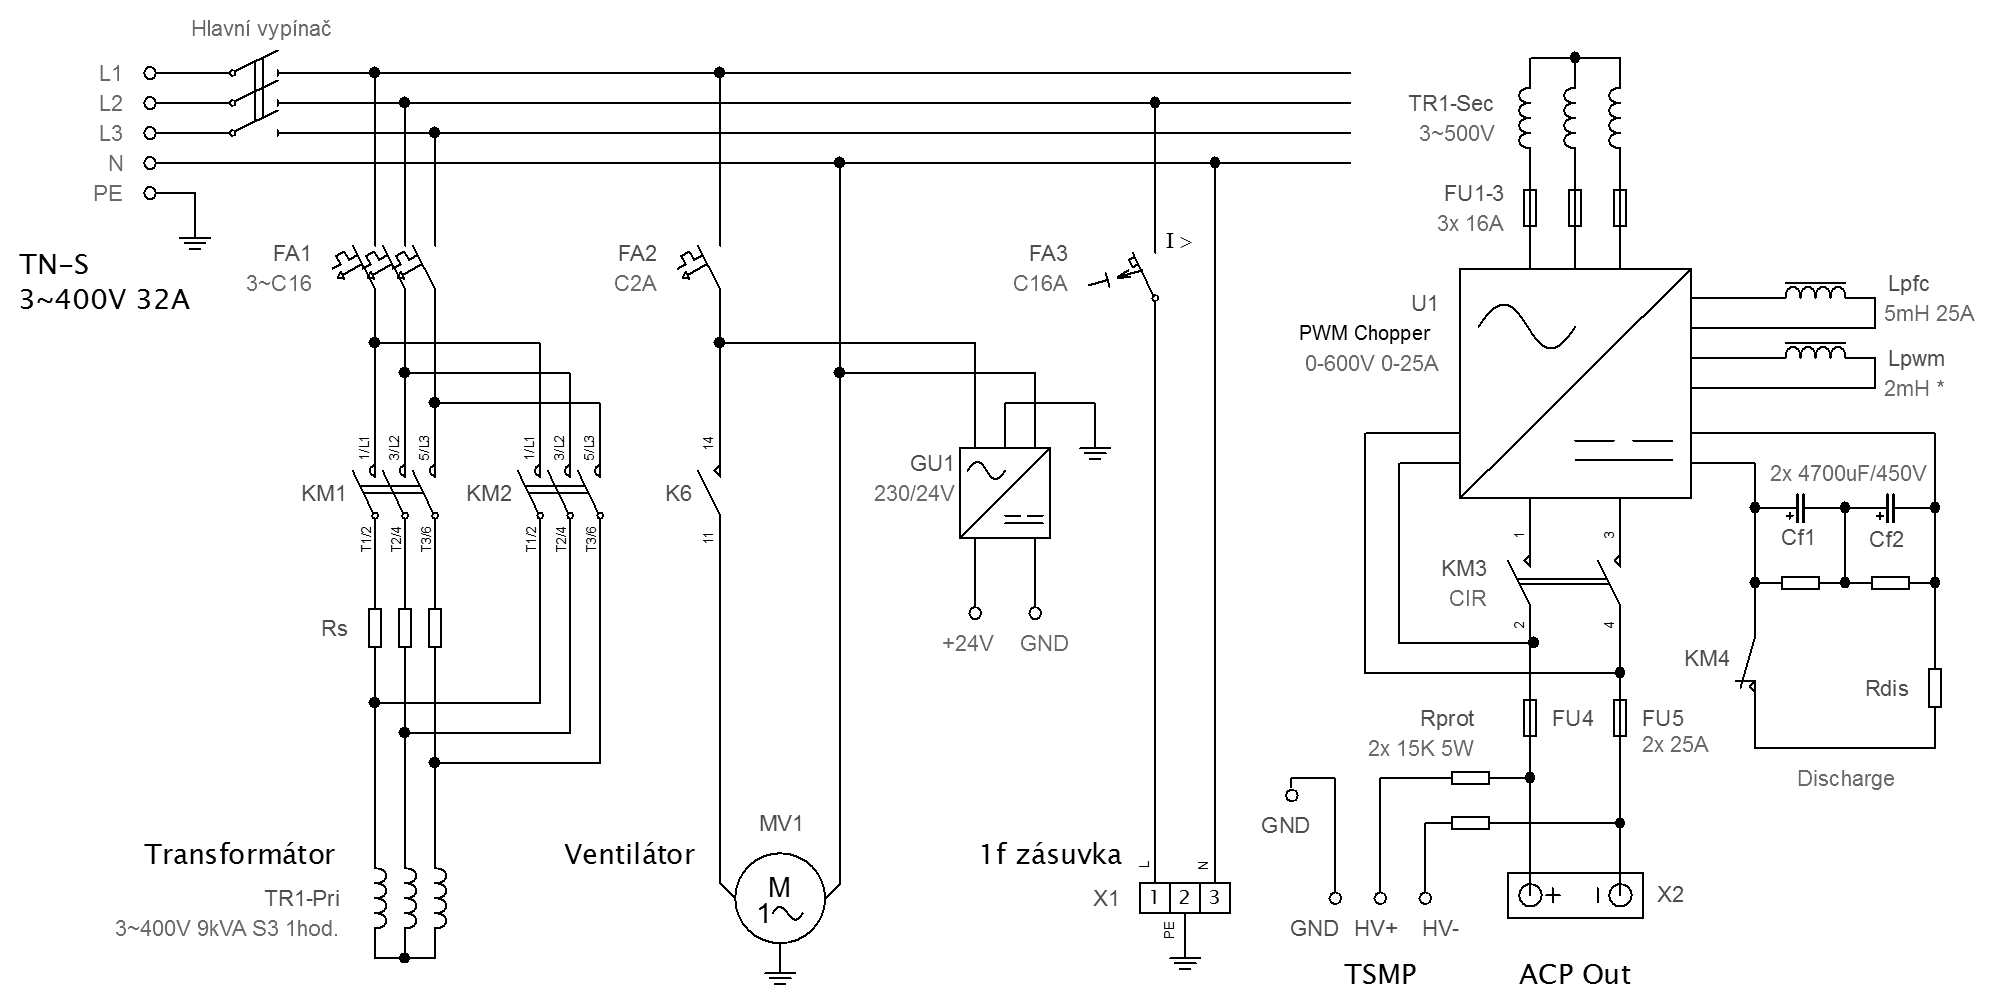
\includegraphics[width=\textwidth]{./img/charger_topology.png}
	\caption{Charger topology.}
	\label{fig:charger_topology}
\end{figure}

\begin{figure}[H]
	\centering
	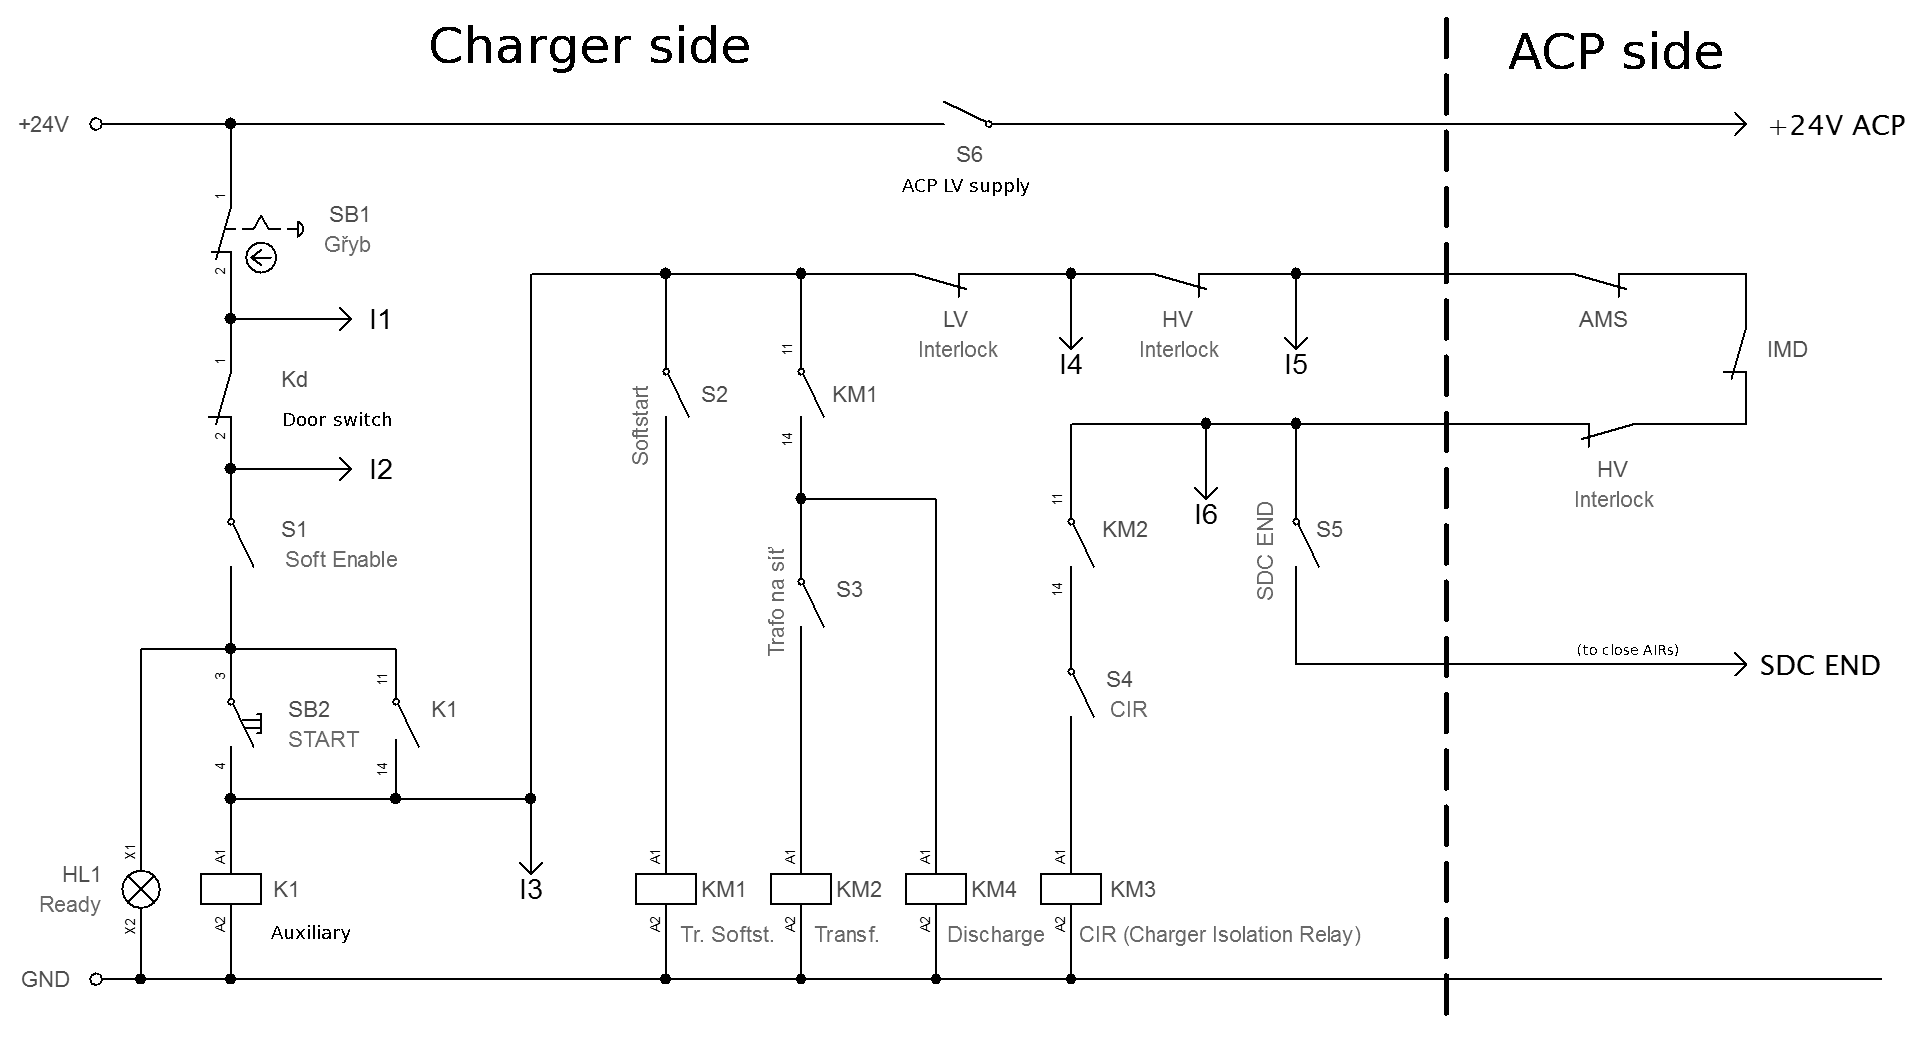
\includegraphics[width=\textwidth]{./img/charger_sdc_schematic.png}
	\caption{Charger SDC scheme.}
	\label{fig:charger_sdc_scheme}
\end{figure}

\begin{figure}[H]
	\centering
	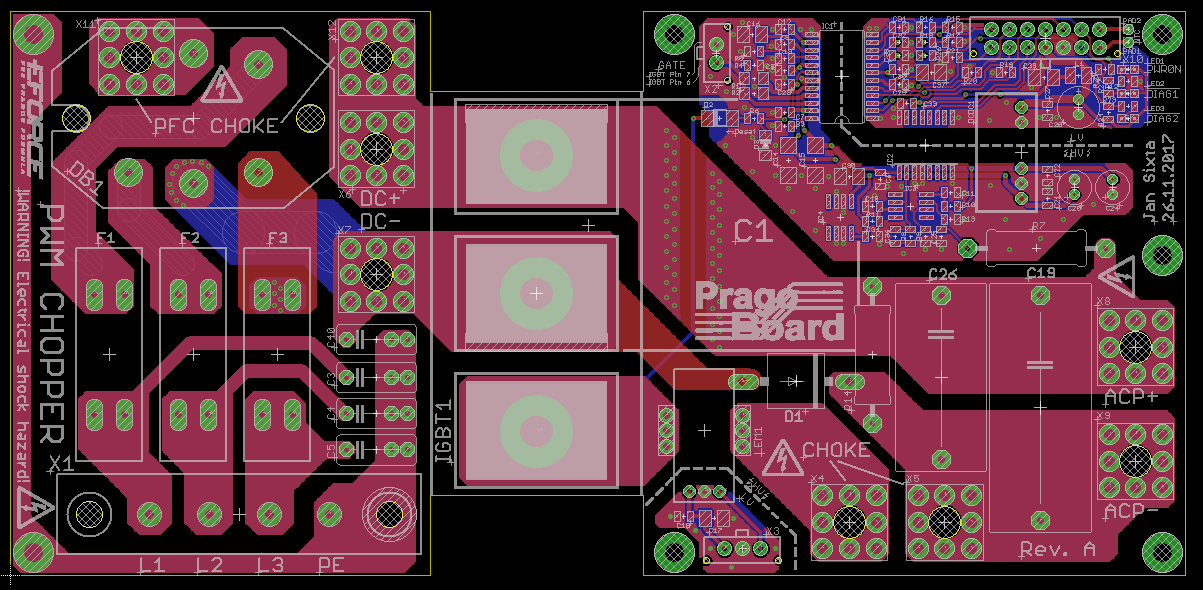
\includegraphics[width=\textwidth]{./img/charger_layout.png}
	\caption{Charger layout.}
	\label{fig:charger_layout}
\end{figure}

\begin{table}[H]
	\centering
	\caption{General charger data}
	\begin{tabu}{|X|X|}
		\hline
		Charger Type: & Self developed charger \\
		\hline
		Maximum charging power: & 9 kVA  \\
		\hline
		Maximum charging voltage: & 600 V \\
		\hline
		Maximum charging current: & 25 A \\
		\hline
		Interface with accumulator & CAN bus \\
		\hline
		Input voltage: & 3x400 V, 50 Hz \\
		\hline
		Input current: & 3x16 A \\
		\hline
	\end{tabu}%
	\label{tab:acc-charger}%
\end{table}%

\subsubsection{Mechanical Configuration/materials}
%Describe the concept of the container, show how the cells are mounted, use CAD-Renderings, show data regarding materials used, etc.

The whole mechanical structure of the case is made from sandwich structure, kevlar fiber and core, designed to be alternative structure. Basically the case is divided to main box, which is outer walls and floor, five longitudinal walls and one transverse wall divided this space on chambers for six stacks and space in front is used for additional technology (\gls{ecu}, \gls{imd}, \glspl{air}, Fuse, Current sensors, connectors etc.). AIR-Box is constructed of FR4 walls. The last component is lid, which is also the stacks holder, you can see in the picture.

Detailed stack composition is shown below in \ref{fig:acp-mech}. Cells are built in a support structure on each side and middle one. There are connecting plates made from welder of Ni201 alloy plate and copper CU99,99\% plate and spot-welded to respective cells. The entire stack is covered with an kevlar case. Each pole of a stack is ended by a copper terminal on the top of the stack. There are also vents hole at the cover and rear outer wall at main wall and also on both sides of stack, cells are cooled by air flowing among them. \gls{bms} board is placed on the top of each stack.

\begin{figure}[H]
	\centering
	\includegraphics[width=\textwidth]{./img/acp-mech.png}
	\caption{Mechanical fastening of \gls{acp}.}
	\label{fig:acp-mech}
\end{figure}

\subsubsection{Position in car}
%Provide CAD-renderings showing the relevant parts. Mark the parts in the rendering, if necessary.  Ensure that the required mechanical structure to protect the accumulator and other electrical components is clearly identified.

\begin{figure}[H]
	\centering
	\includegraphics[width=\textwidth]{./img/acp-position.jpg}
	\caption{Position of \gls{acp} in car.}
	\label{fig:ACP-position}
\end{figure}

